\chapter{Trabajo relacionado}\label{cap:conclusiones}
\noindent El presente cap\'itulo describe otras soluciones particulares para la ejecuci\'on de algoritmia MapReduce. Exploraremos brevemente las caracter\'isticas de cada uno de ellos realizando una comparaci\'on con la soluci\'on propuesta en este proyecto.


\section{Amazon Elastic MapReduce}\label{sec:emc}
\noindent \emph{Elastic MapReduce} \cite{aws} es un servicio web gestionado por Amazon que permite al usuario enviar peticiones de ejecuci\'on de trabajos escritos seg\'un el paradigma MapReduce. EMR se apoya directamente en otro servicio de Amazon, el ya conocido EC2, para abastecer bajo demanda la infraestructura requirida por el trabajo MapReduce.
Dicho de otra forma, el usuario de EMR no tendr\'a que preocuparse por aprovisionar infraestructura, crear, con\-fi\-gu\-rar o destruir las m\'aquinas virtuales que soportan la ejecuci\'on, o afinar la instalaci\'on del framework MapReduce ---Hadoop hasta ahora. Esta conveniente transparencia, sin embargo, lleva impl\'icitas una serie de limitaciones importantes:

\begin{description}
 \item[Restricci\'on de infraestructura:] al ser un servicio otorgado por Amazon, era esperable que la utilizaci\'on de recursos hardware fuera de su control estuviese limitado; y as\'i es: los usuarios de EMR no est\'an habilitados a acoplar sus m\'aquinas virtuales a otros clouds cuyo coste de explotaci\'on pudiera ser m\'as bajo o gratuito.
 Nuestra aproximaci\'on, como se ha visto, segrega y expone las responsabilidades, de tal forma que utilizar un cloud distinto a OpenStack, por ejemplo, s\'olo requiere adaptar el m\'odulo \texttt{Compute} a la sintaxis del API REST del cloud concreto que se utilice.
 \item[Restricci\'on de instalaci\'on:] no es posible usar una m\'aquina virtual personal para ejecutar nuestra propia configuraci\'on de Hadoop en EMR. Nosotros hemos reducido la personalizaci\'on \emph{incrustada} en la m\'aquina virtual Hadoop con un doble objetivo:
   \begin{itemize}
    \item Primero, desacoplar la configuraci\'on para facilitar actualizaciones de kernel, Hadoop, JRE, etc., pas\'andola a Fabric. De tal forma que cuando se pretenda actualizar Hadoop, s\'olo sea necesario reescribir los nuevos \texttt{core-site.xml}, \texttt{mapred-site.xml} y \texttt{hdfs-site.xml} con los antiguos.
    \item Segundo, abrir la posibilidad de integrar soluciones personales de Hadoop, es decir, instalaciones de Hadoop sobre otros sistemas operativos o sobre otras implementaciones de Java, por ejemplo. De nuevo s\'olo requiriendo que se conserven los esqueletos de los ficheros de configuraci\'on mencionados.
   \end{itemize}
 \item[Restricci\'on de informaci\'on:] algunos usuarios estar\'an bajo contratos de confidencialidad que impedir\'an que los datos sean compartidos con terceros como Amazon, haciendo imposible la explotaci\'on del servicio. En nuestro caso, el c\'odigo fuente est\'a liberado y las herramientas empleadas para modificar el proyecto est\'an disponibles sin coste en Internet. Esto abre la posibilidad de organizar despliegues personalizados haciendo m\'inimas alteraciones al c\'odigo presentado.
\end{description}

La tipolog\'ia de los nodos desplegados presenta ciertas peculiaridades que describimos a continuaci\'on. Un cl\'uster EMR tiene tres tipos de nodos:

\begin{description}
 \item[Master:] el nodo maestro, \'unico en sus despligues, ejecuta tanto \emph{NameNode} como \emph{JobTracker}.
 \item[Core:] los nodos n\'ucleo almacenan informaci\'on y procesan tareas. Est\'an compuestos, b\'asicamente, por un \emph{DataNode} y un \emph{TaskTracker}.
 \item[Task:] los nodos tarea s\'olo corren \emph{TaskTrackers}.
\end{description}

Los clusters desplegados por nuestro proyecto configuran, por defecto, un nodo maestro y esclavo al mismo tiempo ---con NameNode, JobTracker, DataNode y TaskTracker--- y el resto se despliegan como esclavos ---nodos \emph{Core} en terminolog\'ia de Amazon. Si bien la configuraci\'on del despligue est\'a fijada en el c\'odigo, resulta muy sencillo alterar las reglas de aprovisionamiento definidas retocando el m\'odulo \texttt{mapred.fabric.fabfile}.\newline

En cuanto al flujo de funcionamiento habitual, EMR posibilita no des\-truir las instancias del cl\'uster cuando \'estas terminen los trabajos programados para evitar la sobrecarga computacional que supone arrancarlas. Nosotros hemos decidido destruir las instancias una vez que se concluye la ejecuci\'on programada. Igualmente, alterar ese comportamiento es sencillo.\newline

En lo que concierne al almacenamiento, EMR se apoya en el S3 de Amazon tanto para cargar los datos de entrada en el flujo de Hadoop, como para escribir los resultados finales. La informaci\'on intermedia se guarda en el HDFS de las m\'aquinas virtuales, que se crea y destruye con las instancias que le dan soporte, eliminando aquella entre ejecuciones. Nuestra aproximaci\'on supone utilizar el sistema de ficheros del nodo en el que resida el servidor web para E/S al cl\'uster Hadoop y de la misma forma nos valemos de HDFS para los resultados intermedios. Hadoop soporta la E/S tambi\'en sobre S3 entre otros; el problema radica en organizar las entradas y salidas al cl\'uster hasta un repositorio externo al sistema de ficheros del nodo. Organizar en sentido global, es decir, no s\'olo disponer la E/S de Hadoop sino tambi\'en actualizar la BD o localizar el fichero para descargar cuando as\'i se requiera desde la interfaz. Django proporciona una implementaci\'on por defecto para gestionar la recogida y el env\'io de ficheros a la web. Esta implementaci\'on se acopla al flujo natural de Django, otorgando la posibilidad de utilizar un adaptador personal para que Django pueda gestionar, del mismo modo, los ficheros alojados en cualquier otro tipo de repositorio.


\section{Resilin}\label{sec:resilin}
\noindent \emph{Resilin} \cite{resilin} pretende mejorar las caracter\'isticas del EMR superando sus li\-mi\-ta\-cio\-nes. El equipo de desarrollo ha escrito un API (ver figura \ref{fig:arquitecturaresilin}) capaz de recibir peticiones con sintaxis EMR que traduce en dos tipos de acciones:
\begin{itemize}
 \item Interacciones con un cloud IaaS para crear y destruir instancias ---que nuestra propuesta maneja con el m\'odulo \texttt{Compute}.
 \item Conexiones SSH a las instancias Hadoop, para configurar y ejecutar las tareas. Nuestro proyecto se apoya en \emph{Fabric} y el m\'odulo \texttt{fabfile} para crear y gestionar los trabajos.
\end{itemize}

\begin{figure}[tbp]
\begin{center}
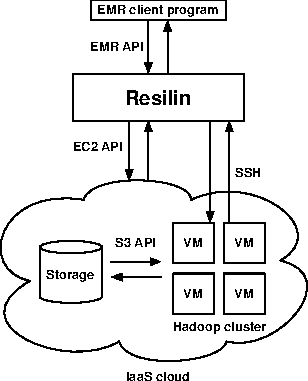
\includegraphics[width=0.5\textwidth]{imagenes/035.pdf}
 \caption{Arquitectura de Resilin. Fuente: \cite{resilin}}
\label{fig:arquitecturaresilin}
\end{center}
\end{figure}

El almac\'en de informaci\'on y la E/S la controlan a trav\'es del API de compatibilidad con S3 que implementan tanto Nimbus como Eucalyptus ---con Cumulus y Walrus respectivamente. Bien es cierto que, como mencionan en \cite{resilin}, tuvieron que realizar ciertas alteraciones en los fuentes.\newline

A mayores, y tal vez lo m\'as interesante de Resilin, se experimenta con la posibilidad de ejecutar flujos de trabajo tomando infraestructura de m\'ultiples clouds. A pesar de no ser la mejor aproximaci\'on en general, debido sobre todo a la dificultad de lidiar la heterogeneidad inherente ---como las diferencias entre instancias virtuales--- y a la sobrecarga de comunicaci\'on introducida. No obstante, s\'i identifican ciertas aplicaciones MapReduce que pudieran verse afectadas favorablemente con esta adici\'on. El modo de proceder elegido para Resilin, que permite conectar nodos virtuales de distintos clouds, consiste en poner en contacto al nodo maestro de un cloud con los esclavos de otro de forma que la comunicaci\'on intercloud sea transparente, tanto para usuarios como para Hadoop.\newline

Nuestra propuesta no soporta la funcionalidad de dirigir trabajos de reducci\'on en distintos clouds. Sin embargo, se podr\'ia ampliar la cobertura retocando el m\'odulo \texttt{Compute}.\newline

En resumen, Resilin presenta la aproximaci\'on m\'as similar a la nuestra de las analizadas, delegando la reducci\'on de los fujos MapReduce en Hadoop y la configuraci\'on del hardware virtual en un cloud cuyo API sea compatible con el de EC2 ---los cuatro evaluados en la secci\'on \ref{sec:frameworksevaluados} lo son. Por \'ultimo, la figura \ref{fig:resilinproyecto} compara las herramientas que soportan la funcionalidad expuesta.

\begin{figure}[tbp]
\begin{center}
\begin{tabular}{|c|c|c|}
\hline
& \textbf{Resilin} & \textbf{Proyecto} \\
\hline
\textbf{Global} & \texttt{Python} & \texttt{Python} \\
\hline
\textbf{HTTP} & \texttt{Twisted} & \texttt{Django} \\
\hline
\textbf{Interacci\'on API cloud} & \texttt{boto} & \texttt{Compute} (m\'odulo propio) \\
\hline
\textbf{Interacci\'on instancias SSH} & \texttt{paramiko} & \texttt{Fabric} \\
\hline
\end{tabular}
\caption{Comparaci\'on de herramientas}
\label{fig:resilinproyecto}
\end{center}
\end{figure}



\section{Cloud MapReduce}\label{sec:cloudmapred}
\noindent \emph{Cloud MapReduce} representa una aproximaci\'on diametralmente opuesta a Resilin. Mientras Resilin pretende implementar un API MapReduce centr\'andose en \emph{organizar} los distintos componentes necesarios, Cloud MapReduce se apoya en los servicios de un cloud ---en concreto el de Amazon--- para implementar el modelo MapReduce \cite{googlemapreduce} \emph{directamente} sobre \'el.\newline

A continuaci\'on comentamos algunas propiedades de Cloud MapReduce que consideramos m\'as relevantes:

\begin{description}
\item[Escalabilidad incremental:] es la capacidad de a\~nadir nuevos nodos al cl\'uster MapReduce cuando el trabajo ya ha comenzado; de tal forma que las nuevas instancias se informen autom\'aticamente del estado global del trabajo y se asignen tareas ellas mismas. Resilin \cite{resilin} lo soporta tambi\'en, nuestro proyecto no.
\item[Simetr\'ia y descentralizaci\'on:] con esta idea se pone manifiesto la falta de jerarqu\'ia en los despligues: cada nodo de un cl\'uster tendr\'a las mismas responsabilidades que sus colegas. Este representa el primer punto de distinci\'on importante frente a las dem\'as aproximaciones ---MapReduce, Hadoop, Amazon EMR, Resilin y nuestro proyecto--- en las que la configuraci\'on, reparto, planificaci\'on, etc. de los trabajos y tareas tiene lugar dentro de los nodos maestro, y la ejecuci\'on y almacenamiento sucede en los esclavos. En Cloud MapReduce los nodos act\'uan de modo independiente, controlando el estado global del trabajo para determinar qu\'e tarea se adec\'ua mejor a las necesidades instant\'aneas del flujo de trabajo. Se debe citar asimismo, que esta simetr\'ia de Cloud MapReduce hace que sea menos problem\'atico superar los problemas en los maestros.
\item[Heterogeneidad:] entendida con una doble componente: por una parte, la posible coexistencia de instancias de distintos \emph{sabores} ---siguiendo la notaci\'on de Amazon--- en un mismo trabajo, y por la otra, la capacidad de crear instancias en m\'ultiples clouds. Resilin soporta ambas cuestiones, nuestra propuesta no.
\end{description}

En Cloud MapReduce el almacenamiento global ---la E/S y los datos intermedios--- se hace sobre S3, la comunicaci\'on y sincronizaci\'on entre nodos con el servicio de colas de Amazon (\emph{SQS} o \emph{Simple Queue Service}) y el almacenamiento de estado de las tareas y nodos en el servicio de base de datos de Amazon, \emph{SimpleDB}. En nuestro proyecto, el almacenamiento global se hace sobre el sistema de ficheros del servidor web; que probablemente no sea la mejor opci\'on debido a las limitaciones de ancho de banda y la falta de tolerancia a fallo. Para modificar este comportamiento, ser\'ia necesario, por ejemplo, dise\~nar un backend de datos personalizado y acoplarlo al \emph{pipe} de almacenamiento de Django, o montar alg\'un sistema de ficheros y apuntar a Django en su direcci\'on. En cuanto a la sincronizaci\'on, comunicaci\'on y estado de las instancias, se delega toda esa funcionalidad en Hadoop.\newline

Por \'ultimo se presenta la figura \ref{fig:arquitecturacloudmapreduce}, que recoge la instant\'anea de alto nivel de un instante de la ejecuci\'on de un trabajo en el Cloud MapReduce. Esta figura recuerda, y no casualmente, a la figura \ref{fig:exmapreduce} que presentaba las fases t\'ipicas de procesamiento del paradigma MapReduce original \cite{googlemapreduce}.

\begin{figure}[tbp]
\begin{center}
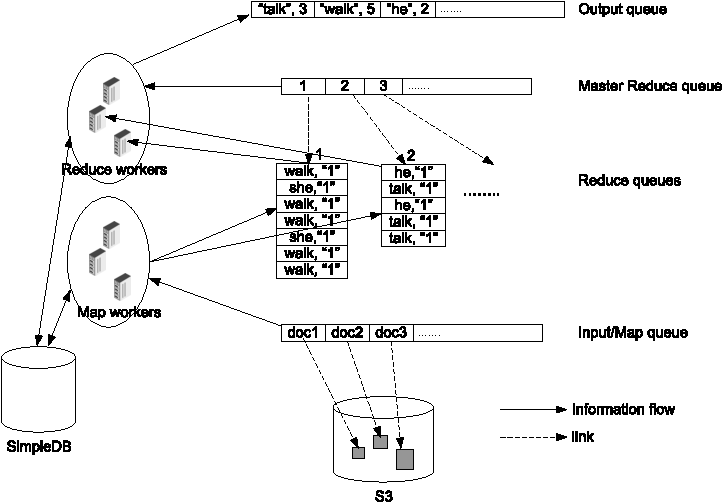
\includegraphics[width=0.9\textwidth]{imagenes/036.pdf}
 \caption{Arquitectura de Cloud MapReduce. Fuente: \cite{cloudmapreduce}}
\label{fig:arquitecturacloudmapreduce}
\end{center}
\end{figure}

\section{Dynamic Cloud MapReduce}\label{sec:dynamicmapreduce}
\hyphenation{SmartFrog}
\noindent La figura \ref{fig:arquitecturadynamicmapreduce} presenta la arquitectura de la soluci\'on propuesta en \cite{dynamicmapreduce} para la apropiaci\'on y configuraci\'on autom\'aticas de infraestructura virtual que procesar\'a aplicaciones MapReduce. Como se ve, los componentes de alto nivel se corresponden directamente con los de nuestra aproximaci\'on; sin embargo (\emph{Dynamic Cloud MapReduce}) presenta algunas diferencias.

\begin{figure}[tbp]
\begin{center}
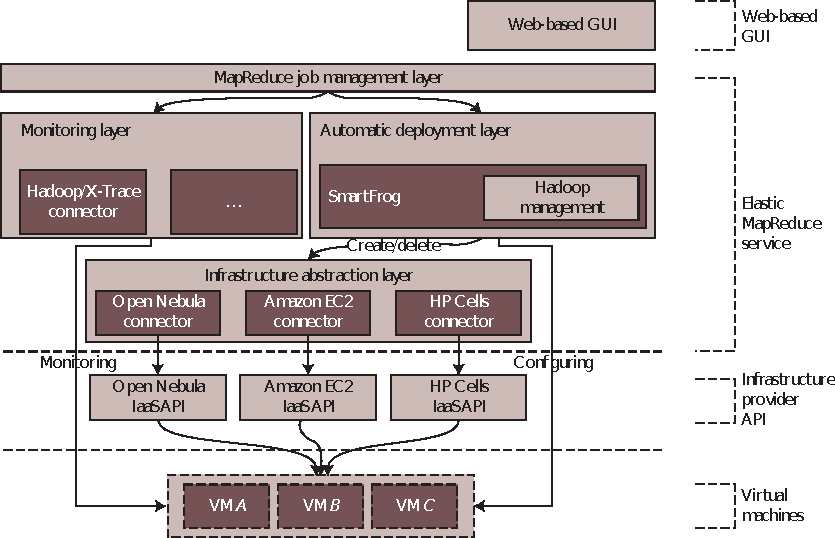
\includegraphics[width=0.9\textwidth]{imagenes/037.pdf}
 \caption{Dynamic Cloud MapReduce. Fuente: \cite{dynamicmapreduce}}
\label{fig:arquitecturadynamicmapreduce}
\end{center}
\end{figure}

\begin{description}
\item[GUI:] a pesar de que la interfaz con el usuario tambi\'en es una p\'agina web, en este caso han implementado un servicio \emph{RESTful} (la capa de direcci\'on de los trabajos MapReduce) que desacopla el manejo del servicio de procesamiento MapReduce. Adem\'as, dicha capa permite que los usuarios del despliegue encadenen la ejecuci\'on de m\'ultiples trabajos MapReduce. En nuestra propuesta hemos implementado las acciones de despliegue y procesado formando parte de la mec\'anica de la web. Este \'ultimo punto, el encadenamiento de flujos MapReduce, no se soporta.
\item[Monitoring Layer:] como su nombre indica, es una capa orientada a la monitorizaci\'on de los procesos MapReduce. Si bien no hemos integrado esta caracter\'istica en la interfaz web, tampoco hemos limitado el acceso a los servicios de monitorizaci\'on integrados en Hadoop; en referencia a los comentados microservidores web de cada m\'odulo \emph{Tracker}.
\item[Automatic Deployment Layer:] con esta capa software se controla el des\-plie\-gue virtual. Equivale a nuestro m\'odulo \emph{Fabric} (\texttt{fabfile.py}). La diferencia fundamental, a parte de que usan \emph{SmartFrog} para gestionar el despliegue, es que la m\'aquina virtual parte de una instalaci\'on \emph{limpia} del sistema operativo a la que se le ha agregado exclusivamente  SmartFrog. De manera que, antes de ejecutar cada flujo MapReduce, SmartFrog gestiona la descarga, instalaci\'on y configuraci\'on de Hadoop en cada m\'aquina virtual. Esta aproximaci\'on es m\'as flexible que la propuesta en el proyecto ---nos apoyamos en una imagen con Hadoop y el JRE preinstalados---, pero a\~nade una importante sobrecarga de descarga y configuraci\'on.
\item[Infrastructure Provider Abstraction Layer:] con esta fachada separan la sintaxis del servicio REST del cloud concreto desplegado, permitiendo definir adaptadores para cada uno. En nuestra propuesta no hemos aislado una interfaz que permita definir adaptadores de forma transparente. Sin embargo, y tal como se ha apuntado, bastar\'ia definir el comportamiento de las funciones del m\'odulo \texttt{Compute} (\texttt{compute.py}) y adaptar los \emph{Transfer Objects} (\texttt{objects.py}) a cada sintaxis.
\end{description}

Por \'ultimo, hacer constar que la opci\'on elegida para el almacenamiento es muy parecida a la propuesta ---\emph{HDFS} y sistema de ficheros local. Sin embargo, nuestra soluci\'on es autom\'atica: no requiere que el usuario suba manualmente los ficheros de entrada. Los ficheros de salida se almacenan en un servidor local y son accesibles desde la interfaz REST. En nuestra propuesta se permite que cada usuario descargue los resultados de sus procesamientos desde la interfaz web.

\section{Resumen}\label{sec:resumenconclusiones}
\noindent Teniendo en cuenta lo expuesto hasta este punto, se podr\'ia pensar que nuestra implementaci\'on es la m\'as limitada. Sin embargo, presenta una importante ventaja frente a todas las dem\'as solucciones: la \emph{absoluta simplicidad}. Lo que parece un car\'acter secundario se convierte en algo fundamental si el usuario es inexperto o si se pretende hacer un despliegue r\'apido de tecnolog\'ia MapReduce el\'astica.\newline

Ninguna de las soluciones estudiadas presenta una aproximaci\'on tan simple e integrada de instalaci\'on, configuraci\'on y explotaci\'on de infraestructura. Todas conllevan alg\'un esfuerzo adicional del usuario, requiriendo, en general: el conocimiento de su mec\'anica interna, el despliegue previo de un cloud, el abono bajo consumo o el hacer p\'ublicos los datos de entrada al framework MapReduce. En resumen, nuestro proyecto es la elecci\'on natural para des\-plie\-gues reducidos inicialmente o como punto introductorio a las tecnolog\'ias cloud IaaS y MapReduce. Partiendo de un despligue m\'inimo y autom\'atico, el administrador del cloud podr\'a agregar nuevos nodos de procesamiento, ac\-tua\-li\-zar la m\'aquina virtual Hadoop, alterar la mec\'anica de aprovisionamiento o, incluso, instalar un cloud de otro proveedor, sin demasiado esfuerzo.
